\documentclass[a4paper,11pt]{report}
\usepackage[utf8]{inputenc}
\usepackage[T1]{fontenc}

%Page margins, header and footer positions
\usepackage{geometry}
 \geometry{
 a4paper,
 total={210mm,297mm},
 left=25mm,
 right=25mm,
 top=30mm,
 bottom=25mm,
 headsep=7mm}

\interfootnotelinepenalty=10000

%To display filling dots in the TOC for all entries
\usepackage[titles]{tocloft}
\renewcommand{\cftsecleader}{\cftdotfill{\cftdotsep}}

%Define new header and footer style
\usepackage{fancyhdr}

\pagestyle{fancy}
\fancyhf{}
\lhead{\color{Gray}{\small{ Best Bike Paths by Luca Suzani, Alberto Spezzapria, Alessio Pesavento}}}
\lfoot{\textcolor{Gray}{\small{Copyright © 2025, Luca Suzani, Alberto Spezzapria, Alessio Pesavento – All rights reserved}}}
\rfoot{\textcolor{Gray}{\thepage}}
\renewcommand{\headrulewidth}{0pt}

%PACKAGES
\usepackage{wasysym}
\usepackage{pifont}

\newcommand{\supported}{\ding{52}\xspace}
\newcommand{\unsupported}{\ding{55}\xspace}
\newcommand{\partsupported}{\textcolor{black!40}{\ding{52}}\xspace}
\newcommand{\lowsupported}{\textcolor{black!20}{\ding{52}}\xspace}
\newcommand{\unknowsupported}{\textbf{?}\xspace}

%Font: Times
\usepackage{times}
%Change monospaced font
\renewcommand{\ttdefault}{lmtt}

%tables
\usepackage{tabu}
\usepackage{tabularx}
\usepackage{ltablex}
\usepackage{longtable}
\usepackage{float} % To allow the use of H modifier in long tables

%landscape mode
\usepackage{pdflscape}
\usepackage{rotating}
\usepackage{caption}

%make landscape mode be sensitive to even and odd pages
%start
\def\myrotate{\ifodd\c@page\else-\fi 90}
\makeatletter
\global\let\orig@begin@landscape=\landscape%
\global\let\orig@end@landscape=\endlandscape%
\gdef\@true{1}
\gdef\@false{0}
\gdef\landscape{%
    \global\let\within@landscape=\@true%
    \orig@begin@landscape%
}%
\gdef\endlandscape{%
    \orig@end@landscape%
    \global\let\within@landscape=\@false%
}%
\@ifpackageloaded{pdflscape}{%
    \gdef\pdf@landscape@rotate{\PLS@Rotate}%
}{
    \gdef\pdf@landscape@rotate#1{}%
}
\let\latex@outputpage\@outputpage
\def\@outputpage{
    \ifx\within@landscape\@true%
        \if@twoside%
            \ifodd\c@page%
                \gdef\LS@rot{\setbox\@outputbox\vbox{%
                    \pdf@landscape@rotate{-90}%
                    \hbox{\rotatebox{90}{\hbox{\rotatebox{180}{\box\@outputbox}}}}}%
                }%
            \else%
                \gdef\LS@rot{\setbox\@outputbox\vbox{%
                    \pdf@landscape@rotate{+90}%
                    \hbox{\rotatebox{90}{\hbox{\rotatebox{0}{\box\@outputbox}}}}}%
                }%
            \fi%
        \else%
            \gdef\LS@rot{\setbox\@outputbox\vbox{%
                \pdf@landscape@rotate{+90}%
                \hbox{\rotatebox{90}{\hbox{\rotatebox{0}{\box\@outputbox}}}}}%
            }%
        \fi%
    \fi%
    \latex@outputpage%
}
\makeatother
%end

%graphics
\usepackage{graphicx}
\usepackage[dvipsnames, table]{xcolor}
%If you upload images from PC, you need to insert code for the path here (different for Windows and Unix OS)

%References
%\usepackage{xpatch}
%\usepackage[backend=biber, style=numeric, citestyle=numeric, sorting=none]{biblatex}
%\addbibresource{main.bib}

%Other
\usepackage{ifthen}
\usepackage{xspace}
\usepackage{enumitem}
\usepackage{amssymb}
% hyperref: hide link colors (prevents red/colored ToC and list entries)
\usepackage[hidelinks]{hyperref}
\newcommand{\comment}[1]{{\color{Red}$\blacktriangleright$ Comment: #1 $\blacktriangleleft$}}


% Some utilities\ldots
\usepackage{soul}
\usepackage{tikz}

\usetikzlibrary{calc}
\usetikzlibrary{decorations.pathmorphing}


\makeatletter

\newcommand{\defhighlighter}[3][]{%
  \tikzset{every highlighter/.style={color=#2, fill opacity=#3, #1}}%
}

\defhighlighter{yellow}{.5}

\newcommand{\highlight@DoHighlight}{
  \fill [ decoration = {random steps, amplitude=1pt, segment length=15pt}
        , outer sep = -15pt, inner sep = 0pt, decorate
       , every highlighter, this highlighter ]
        ($(begin highlight)+(0,8pt)$) rectangle ($(end highlight)+(0,-3pt)$) ;
}

\newcommand{\highlight@BeginHighlight}{
  \coordinate (begin highlight) at (0,0) ;
}

\newcommand{\highlight@EndHighlight}{
  \coordinate (end highlight) at (0,0) ;
}

\newdimen\highlight@previous
\newdimen\highlight@current

\DeclareRobustCommand*\highlight[1][]{%
  \tikzset{this highlighter/.style={#1}}%
  \SOUL@setup
  %
  \def\SOUL@preamble{%
    \begin{tikzpicture}[overlay, remember picture]
      \highlight@BeginHighlight
      \highlight@EndHighlight
    \end{tikzpicture}%
  }%
  %
  \def\SOUL@postamble{%
    \begin{tikzpicture}[overlay, remember picture]
      \highlight@EndHighlight
      \highlight@DoHighlight
    \end{tikzpicture}%
  }%
  %
  \def\SOUL@everyhyphen{%
    \discretionary{%
      \SOUL@setkern\SOUL@hyphkern
      \SOUL@sethyphenchar
      \tikz[overlay, remember picture] \highlight@EndHighlight ;%
    }{%
    }{%
      \SOUL@setkern\SOUL@charkern
    }%
  }%
  %
  \def\SOUL@everyexhyphen##1{%
    \SOUL@setkern\SOUL@hyphkern
    \hbox{##1}%
    \discretionary{%
      \tikz[overlay, remember picture] \highlight@EndHighlight ;%
    }{%
    }{%
      \SOUL@setkern\SOUL@charkern
    }%
  }%
  %
  \def\SOUL@everysyllable{%
    \begin{tikzpicture}[overlay, remember picture]
      \path let \p0 = (begin highlight), \p1 = (0,0) in \pgfextra
        \global\highlight@previous=\y0
        \global\highlight@current =\y1
      \endpgfextra (0,0) ;
      \ifdim\highlight@current < \highlight@previous
        \highlight@DoHighlight
        \highlight@BeginHighlight
      \fi
    \end{tikzpicture}%
    \the\SOUL@syllable
    \tikz[overlay, remember picture] \highlight@EndHighlight ;%
  }%
  \SOUL@
}

\makeatother

% Common abbrev. are set as commands to ensure proper spacing after the dot
\RequirePackage{xspace}
\newcommand{\ie}{i.e.\@\xspace}
\newcommand{\aka}{a.k.a.\@\xspace}
\newcommand{\Ie}{I.e.\@\xspace}
\newcommand{\cf}{cf.\@\xspace}
\newcommand{\Cf}{Cf.\@\xspace}
\newcommand{\eg}{e.g.\@\xspace}
\newcommand{\Eg}{E.g.\@\xspace}
\newcommand{\etal}{et al.\@\xspace}
\newcommand{\etc}{etc.\@\xspace}
\newcommand{\wrt}{w.r.t.\@\xspace}
\newcommand{\Wrt}{W.r.t.\@\xspace}



\date{}

\usepackage{multirow}

\usepackage{listings}
\usepackage{xcolor}

% Definizione colori per il codice
\definecolor{codegreen}{rgb}{0,0.6,0}
\definecolor{codegray}{rgb}{0.5,0.5,0.5}
\definecolor{codepurple}{rgb}{0.58,0,0.82}
\definecolor{backcolour}{rgb}{0.95, 0.95, 0.95}

% Definizione del linguaggio Alloy per evidenziazione sintassi
\lstdefinelanguage{Alloy}{
    keywords={module, sig, enum, fact, pred, assert, run, check, for, but, Int, one, lone, set, seq, extends, in, disj, all, some, no, implies, else, let, sum},
    keywordstyle=\color{blue}\bfseries,
    ndkeywords={True, False, Optimal, Sufficient, Bad, Private, Public},
    ndkeywordstyle=\color{codepurple}\bfseries,
    identifierstyle=\color{black},
    sensitive=true,
    comment=[l]{--},
    morecomment=[l]{//},
    morecomment=[s]{/*}{*/},
    commentstyle=\color{codegreen}\ttfamily,
    stringstyle=\color{red}\ttfamily,
    morestring=[b]",
}

% Stile generale del blocco codice
\lstset{
    backgroundcolor=\color{backcolour},   
    basicstyle=\ttfamily\footnotesize,
    breakatwhitespace=false,         
    breaklines=true,                 
    captionpos=b,                    
    keepspaces=true,                 
    numbers=left,                    
    numbersep=5pt,                  
    showspaces=false,                
    showstringspaces=false,
    showtabs=false,                  
    tabsize=2,
    frame=single
}

\begin{document}

%TITLE PAGE

\begin{titlepage}


%LOGO

{\begin{table}[t!]
\centering
\begin{tabu} to \textwidth { X[1.3,r,p] X[1.7,l,p] }
\textcolor{Blue}
{\textbf{\small{Best Bike Paths, Luca Suzani, Alberto Spezzapria, Alessio Pesavento}}} & 
\includegraphics[scale=0.5]{Images/PolimiLogo}
\end{tabu}
\end{table}}~\\ [7cm]

%TITLE 

\begin{flushleft}

%Replace the text string with your title
{\textcolor{Blue}{\textbf{\Huge{Requirement Analysis and Specification
        Document}}}} \\ [1cm]

\end{flushleft}

\end{titlepage}

%Define deliverable specific info
%Replace cell contents where needed
\begin{table}[h!]
\begin{tabu} to \textwidth { X[0.3,r,p] X[0.7,l,p] }
\hline

\textbf{Deliverable:} & RASD\\
\textbf{Title:} & Requirement Analysis and Verification Document \\
\textbf{Authors:} & Luca Suzani, Alberto Spezzapria, Alessio Pesavento \\
\textbf{Version:} & 1.0 \\ 
\textbf{Date:} & 22-December-2025 \\
\textbf{Download page:} & https://github.com/Alessio01103/PesaventoSpezzapriaSuzani.git \\
\textbf{Copyright:} & Copyright © 2025, Luca Suzani, Alberto Spezzapria, Alessio Pesavento – All rights reserved \\
\hline
\end{tabu}
\end{table}




\setcounter{page}{2}


%------------------------------------------------------------------------------------------------------------------------------------------------
\newpage
\addcontentsline{toc}{section}{Table of Contents}
\tableofcontents
\newpage
\addcontentsline{toc}{section}{List of Figures}
\listoffigures
\addcontentsline{toc}{section}{List of Tables}
\listoftables

%------------------------------------------------------------------------------------------------------------------------------------------------
\clearpage
\chapter{{Introduction}}
\label{sect:introduction}
\section{Purpose}
The purpose of the \textit{Best Bike Paths (BBP)} system is to promote cycling as a sustainable, safe, and conscious means of transportation by providing cyclists with a digital platform for collecting, accessing, and sharing information about cycling routes and activities.\\
The system addresses the need for reliable and up-to-date data on bike paths, allowing users to track their performance while contributing to the improvement of shared information.\\
Through active community participation, BBP aims to identify and maintain the safest and most efficient routes, fostering a more informed and widespread cycling mobility.\\
Ultimately, BBP seeks to enhance the overall cycling experience by integrating multiple functionalities and creating a collaborative, continuously updated information network driven by user contributions.\\

\subsection{Goals}
\begin{enumerate}[label=G\arabic*.]
\item \textbf{Support cyclists in tracking their activities:} Enable users to record their cycling routes and access detailed statistics such as total distance, average speed, and other performance indicators, enriched, when available, by meteorological data from external services (weather conditions, temperature and wind speed).
\item \textbf{Allow cyclists to contribute information about bike paths:} Provide two modes for entering information related to bike paths:
\begin{itemize}
    \item \textbf{Manual mode:} the user manually inputs the path data and its condition.
    \item \textbf{Automatic mode:} the system automatically collects data via GPS, accelerometer, and gyroscope during the cycling activity, requiring user confirmation before publication.
\end{itemize}

\item \textbf{Enable the publication of recorded path information:} Allow users to make their recorded path information public, contributing to a shared and valuable database for the entire cycling community.
\item \textbf{Enable route search and visualization:} Allow users to search for and display on a map one or more cycling routes connecting a chosen origin and destination, ranking them based on overall condition and effectiveness in reaching the goal.
\item \textbf{Maintain up-to-date and reliable path information:} Ensure continuous updating of path data through the aggregation and analysis of user feedback, taking into account data freshness, consistency among reports, and user confirmations.
\end{enumerate}
\section{Scope}
The main goal of the \textit{Best Bike Paths (BBP)} system is to provide cyclists with a mobile application that allows them to record their activities and share information about bike routes, while also fostering the creation of an active and collaborative community.
The application enables registered users to save their rides, view detailed statistics such as total distance covered or average speed, and contribute to updating the path inventory by reporting the condition of routes or the presence of potential obstacles.
The information entered by users can be made public and is then aggregated by the system, which combines data from multiple sources to offer a comprehensive and up-to-date representation of the paths’ conditions.
Unregistered users can still take advantage of the consultation features by searching for routes between two points and viewing the available options on a map, ranked according to a score that considers both the quality and effectiveness of the routes.
The system also interacts with an external meteorological service, which provides weather data to enrich the information related to recorded activities.

\subsection{World Phenomena}

\subsection{Shared Phenomena}
\section{Definitions, Acronyms, and Abbreviations}
\subsection{Acronyms}
\begin{itemize}
    \item \textbf{BBP:} Best Bike Paths
    \item \textbf{DB:} DataBase
\end{itemize}
\section{Revision History}
Version 1.0: 20/12/2025
\section{Reference Documents}
\begin{itemize} 
    \item \textbf{RDO:} "Best Bike Paths" – Software Engineering 2 Project Assignment, A.Y. 2025-2026, Politecnico di Milano. 
    \item \textbf{UML:} OMG Unified Modeling Language (UML), Version 2.5.1. 
    \item \textbf{Alloy:} Jackson, Daniel. "Software Abstractions: Logic, Language, and Analysis." MIT Press. 
    \item \textbf{GDPR:} Regulation (EU) 2016/679 (General Data Protection Regulation). 
\end{itemize}

\section{Document Structure}
The following list provides a brief overview of the contents of each chapter in this document:

\begin{itemize}
    \item \textbf{Chapter 1 Introduction:} A brief description of the project that follows from the analysis of the specification provided; it highlights the goals of the product and its scope.
    
    \item \textbf{Chapter 2 Overall Description:} A more detailed description of the product that comprehends also real world scenarios and analyses the system from a technical point of view.
    
    \item \textbf{Chapter 3 Specific Requirements:} A detailed list of all the requirements needed in order to satisfy the goals, and their relationship with domain assumptions.
    
    \item \textbf{Chapter 4 Formal analysis using Alloy:} A formal description of a portion of real world phenomena analyzed through Alloy in order to highlight inconsistencies between assumptions and phenomena previously modelized.
    
    \item \textbf{Chapter 5 Effort spent:} The time spent by each member of the group to contribute to the realization of this document.
    
    \item \textbf{Chapter 6 References:} Reference to documents or tools used for writing this document.
\end{itemize}
%what you write here is a comment that is not shown in the final text

%------------------------------------------------------------------------------------------------------------------------------------------------
\clearpage
\chapter{{Overall Description}}
\label{sect:overview}
\section{Product Overview}
\subsection{Scenarios}
\subsubsection*{User publishes a path}
\begin{enumerate}
    \item The user accesses the BBP system and opens the “My Routes” section.
    \item The system displays the list of paths associated with the user, indicating for each one, among other properties, its status (private or public).
    \item The user selects a private route and, using the appropriate button, requests its publication.
    \item Upon receiving the publication request, the system asks the user to confirm additional information related to the route:
        \begin{itemize}
            \item In the case of manually created routes, the user can review and, if necessary, modify the additional information previously entered during creation.
            \item In the case of automatically generated routes, the user must confirm or correct the acquired information (if not already done) and may add further details manually.
        \end{itemize}
    \item Once the review is complete, the user confirms the publication of the route.
    \item The system verifies the data consistency, assigns a unique identifier to the route, and makes it available to the community within the search and browsing functionality.
    \item The system notifies the user of the successful publication and updates the route status from private to public.
\end{enumerate}
\subsubsection*{User modifies the additional information related to a route}
\begin{enumerate}[label=\arabic*.]
    \item The user accesses the Best Bike Paths (BBP) platform and opens the “My Routes” section.
    \item The system displays the list of routes associated with the user, indicating for each one, among other properties, its status (private or public).
    \item The user selects a route and opens the section dedicated to additional information.
    \item The system displays the current information, including:
        \begin{itemize}
            \item The condition of the roads that make up the route;
            \item The presence of obstacles or damaged sections;
            \item The origin of each piece of data (manually entered or automatically acquired).
        \end{itemize}

    \item The user can modify, correct, or add new information:
        \begin{itemize}
            \item If the route was created manually, the user can freely update existing data.
            \item If the route was created automatically, the user can review the information acquired by the system and/or add new data manually; in any case, they must confirm or correct the automatically acquired information before publication.

        \end{itemize}
    \item The system saves the changes and updates the database.




\end{enumerate}

\section{Product Functions}
\subsection*{Sign-Up and Login}
\subsubsection*{Sign-Up}
The system lets the users register in order to manage and record data associated with each of them. When the user accesses the sign-up page for the first time, he’s offered the option to log-in with one of their existing accounts through an OAuth service. This way, his BBP account is linked to another account that he owns, making it easier to remember and access for him. 
The system also gives the user the possibility of entering his email and a new password and to create an account directly inside BBP. In that case, BBP checks that the password is complex enough and that no other account is associated with the same email. If the checks pass, the system stores the information in the DB and grants the user access to the platform.
\subsubsection*{Login}
If the user already has a BBP account or has previously linked their BBP account to one of the other existing accounts that he has through OAuth, the system grants them access the page. If the user access the page through OAuth, a button redirects them to the external account provider’s website, which handles the login process and sends the user back only when he completes the login procedure. If, on the other hand, the user registered directly on BBP, the system first checks whether an account associated with the provided email, and then verifies that the password matches. If thats the case the user is redirected to the website’s homepage.
\subsubsection*{Accessing BBP without accounts}
The user can also access BBP without logging in. In this case, the functionalities that are available are more limited. The system lets the user browse between public paths, but all the recording features and the private paths needs the login to work

\subsection*{Activity Recording}

\subsection*{Entering route condition information}
Each route, whether derived from an automatically recorded activity or manually created by the user, is characterized by a set of additional information describing its condition and rideability.
In particular, this information concerns:
\begin{itemize}
    \item{The condition of the roads that make up the route;}
    \item{The presence of obstacles, such as potholes, surface damage, or dangerous sections.}
\end{itemize}
Additional information is always managed through the same interface, but with different behavior depending on how the route was created:
\begin{itemize}
    \item{\textbf{Manual mode} During route creation, the user directly enters information about the condition of the roads and any obstacles.}
    \item{\textbf{Automatic mode} The system acquires data via the device’s sensors (GPS, accelerometer, gyroscope); therefore, the user finds this information already filled in. Each piece of information must be confirmed.}
\end{itemize}
Regardless of the mode, the user can always modify or update the additional information before and after publication, thus contributing to improving the quality of shared data.

\subsection*{Paths publication}
Registered users can choose to publish a route, making it visible and accessible to other users within the platform.
In particular, publication adds the route to \textit{BBP}’s public archive, making it available to all other users, including non-registered ones, through the route search and browsing functionality. Only published routes can be viewed by others and contribute to enhancing the quality of shared community data.
Publication always concerns the complete route, including all additional information such as road conditions and the presence of any obstacles.

\subsection*{Merging information from different users}
When multiple users provide information regarding the same route or overlapping sections, the BBP system automatically merges the received data concerning road conditions and the presence of obstacles. The merging process takes into account two main factors:
\begin{itemize}
    \item{The freshness of the information, meaning how recently it was provided;}
    \item {The number of confirmations received from different users for the same condition or status.}
\end{itemize}
In the case of conflicting reports, the system applies a weighted evaluation mechanism that prioritizes the most recent and most frequently confirmed information.


\section{User Characteristics}
\subsection{Registered User}
A registered user has a personal profile containing the information provided during registration, the saved paths, and the cycling activities they have performed.
They can save their rides, view detailed statistics (such as distance, average speed, and total time), and contribute to updating the path inventory by reporting the condition of the routes or the presence of obstacles.
The registered user can also create new paths, either manually by entering data directly or automatically during an activity, using the sensors of their mobile device.
After creation, the user can make these paths publishable, allowing the community to access and view them.
Finally, the user can search for bike paths between two points and view them on the map, ordered according to the score assigned by the system.

\subsection{Unregistered User}
An unregistered user can access a limited version of the application, which only allows the consultation of publishable paths available on the platform.
They can search for paths between two points, display them on the map, and view basic information such as the name, score, and general condition of each path, but they cannot perform any additional actions on them.

%------------------------------------------------------------------------------------------------------------------------------------------------
\clearpage
\chapter{{Specific Requirements}}
\label{sect:requirements}
\section{External Interface Requirements}
\section{Functional Requirements}
\subsubsection*{Sign-Up and Login}
\begin{enumerate}
    \item The platform allows users to create an account by providing the required personal information.
    \item The platform allows registered users to log in and access the system.
    \item The platform allows registered users to recover the access credentials.
    \item The platform allows guest users (non-registered users) to access only the path search functionality of the system.
\end{enumerate}
\subsubsection*{Path search from origin to destination}
\begin{enumerate}
    \item The platform allow users to search for cycling paths based on a starting point and an ending point.
    \item The platform allow users to filter the search results based on the path parameters.
\end{enumerate}
\subsubsection*{Path Ranking}
\begin{enumerate}
    \item The platform is able to rank the available paths based on the path data, including the condition of each segment, the freshness of the information, and the effectiveness of the path in connecting the selected points.
\end{enumerate}
\subsubsection*{Entering path condition information}
\begin{enumerate}
    \item The platform is able to detect when a registered user follows a path that is already available to the public and associate the activity with that path.
    \item The platform allow registered users to update the condition information of a path, even without performing an activity on that path.
\end{enumerate}
\section{Performance Requirements}
The Best Bike Paths (BBP) system must ensure high performance to guarantee a smooth user experience and reliable tracking reliability. Regarding response time, the backend must compute path scores and visualize routing results within 3 seconds for 95\% of requests, supporting a concurrent load of at least 1,000 active users. On the mobile client side, energy efficiency is a critical requirement: during 'Automated mode', the combined use of GPS and sensors must not exceed a battery consumption rate of 15\% per hour on standard devices. Finally, to ensure the relevance of shared information (data freshness), path status updates derived from community reports must be propagated and visible to users within 15 minutes of processing.
\section{Design Constraints}
\subsection{Standards Compliance}
\begin{itemize}
    \item \textbf{GDPR Compliance (EU 2016/679):} Since the system collects and processes sensitive personal data (specifically geolocation history and user performance metrics), the architecture must be fully compliant with the General Data Protection Regulation (GDPR). This requires the implementation of explicit consent mechanisms, data anonymization where possible, and the "Right to be Forgotten".
    \item \textbf{ISO/IEC 27001 (Information Security):} The system design must adhere to ISO/IEC 27001 principles for Information Security Management. This constrains the architecture to include mandatory security controls, such as end-to-end encryption (TLS/WSS) for data in transit and encryption for sensitive data at rest.
    \item \textbf{Geospatial Standards (WGS84 \&\ GPX):} To guarantee global interoperability and compatibility with external mapping services, all geospatial coordinates must be stored using the WGS84 reference system. Additionally, data portability for bike paths must support the GPX (GPS Exchange Format) standard.
    \item \textbf{Mobile UI/UX Guidelines:} The mobile application client must strictly follow the Human Interface Guidelines (for iOS) and Material Design principles (for Android). This ensures a user experience that is consistent with the native operating system environment.
\end{itemize}
\subsection{Hardware Limitations}
\begin{itemize}
    \item \textbf{Sensor Suite Requirements:} The availability of the "Automated Mode" is strictly bound by the hardware capabilities of the user's device. The application requires the mandatory presence of:
    \begin{itemize}
        \item A functional GNSS/GPS Receiver.
        \item An Accelerometer.
        \item A Gyroscope.
    \end{itemize}
    \item \textbf{Operating System Compatibility:} To ensure the reliability of sensor data collection (GPS, Accelerometer, Gyroscope) and compliance with modern security standards for background location tracking, the client application must support:
    \begin{itemize}
        \item Android: Version 10.0 (API Level 29) or higher (covering approx. 89\%\ of the active market).
        \item iOS: Version 15.0 or higher (covering approx. 90\%\ of the active market).
    \end{itemize}
\end{itemize}
\subsection{Any other Constraint}
\begin{itemize}
    \item \textbf{Safety \&\ Distraction-Free UI:} To comply with traffic safety regulations and ensure user well-being, the "Automated Mode" interface must be designed as interaction-free. The application shall not prompt for user input or require manual interaction while the device detects that the user is cycling.
\end{itemize}

%------------------------------------------------------------------------------------------------------------------------------------------------
\clearpage
\chapter{{Formal Analysis Using Alloy}}
\label{sect:alloy}
\begin{lstlisting}[language=Alloy, caption={Complete Alloy Model for BestBikePaths}, label={lst:alloy_model}]
module BestBikePathsUnified

/* ==============================================================================
   1. DATA TYPES AND ENUMERATIONS
   Defines basic domains: geographic locations, visibility states, 
   road surface conditions, and boolean values for flags.
   ============================================================================== */
sig Location {}

enum PathStatus { Private, Public }
enum Condition { Optimal, Sufficient, Bad }
enum Bool { True, False }

/* ==============================================================================
   2. SYSTEM ACTORS
   The User is the central entity who owns activities (recordings), 
   paths (publications), and leaves feedback.
   ============================================================================== */
sig User {
    myActivities: set Activity,
    myPaths: set Path,
    myFeedbacks: set Feedback
}

/* ==============================================================================
   3. CORE ENTITIES
   ============================================================================== */

/* ENTITY: ACTIVITY (Sensing/Partner Logic)
   Represents raw sensor data recording.
   - trace: the GPS sequence.
   - avgSpeed: used to filter if the activity is actually "biking".
   - sensorAnomalies: potholes automatically detected by accelerometer.
*/
sig Activity {
    owner: one User,
    trace: seq Location,
    avgSpeed: Int,
    sensorAnomalies: set Location
}

/* ENTITY: PATH (Structure and Publishing Logic)
   Represents the consolidated path in the system.
   - trajectory: the geometry of the path.
   - status/isConfirmed: manage the lifecycle (draft -> public).
   - currentCondition: the aggregated state of the path quality.
*/
sig Path {
    owner: one User,
    trajectory: seq Location,
    status: one PathStatus,
    isConfirmed: one Bool,
    currentCondition: one Condition,
    receivedFeedbacks: set Feedback
}

/* ENTITY: FEEDBACK (Community Logic)
   Represents user opinion on a public path.
   Links an author to a target path, specifying conditions and localized obstacles.
*/
sig Feedback {
    author: one User,
    targetPath: one Path,
    reportedCondition: one Condition,
    reportedObstacles: set Location
}

/* ==============================================================================
   4. FACTS (INVARIANTS AND DOMAIN RULES)
   ============================================================================== */

/* FACT: STRUCTURAL CONSISTENCY
   Ensures bidirectional relationships are consistent (e.g., if feedback 
   belongs to a user, it must appear in that user's feedback list) 
   and establishes ownership hierarchy.
*/
fact StructuralConsistency {
    all a: Activity | a in a.owner.myActivities
    all p: Path | p in p.owner.myPaths
    all f: Feedback | f in f.author.myFeedbacks
    all f: Feedback | f in f.targetPath.receivedFeedbacks
}

/* FACT: GEO CONSISTENCY
   Constrains spatial data:
   1. Obstacles reported in feedback must be on the path trajectory.
   2. Anomalies detected by sensors must be on the activity trace.
   Note: .elems converts the sequence to a set for inclusion check.
*/
fact GeoConsistency {
    all f: Feedback | f.reportedObstacles in f.targetPath.trajectory.elems
    all a: Activity | a.sensorAnomalies in a.trace.elems
}

/* FACT: UNIQUE FEEDBACK (Anti-Spam)
   A user can leave at most one feedback per specific path.
   This prevents ranking manipulation by a single actor.
*/
fact UniqueFeedback {
    all p: Path, u: User | lone f: p.receivedFeedbacks | f.author = u
}

/* FACT: ACTIVITY VALIDATION LOGIC (Sensing)
   Defines rules for an activity to become a path:
   If a path is generated from an activity (sharing owner and trace),
   then the average speed must be compatible with biking 
   (here defined between 4 and 12 to stay within Alloy's small integer range).
*/
fact ActivityToPathLogic {
    all p: Path, a: Activity | 
        (p.trajectory = a.trace and p.owner = a.owner) implies {
            a.avgSpeed > 4 
            a.avgSpeed < 12
    }
}

/* FACT: PRIVATE PATH PRIVACY
   If a path is set to Private, no one except the owner can leave feedback 
   or interact with it.
*/
fact PrivatePathPrivacy {
    all f: Feedback | 
        f.targetPath.status = Private implies f.author = f.targetPath.owner
}

\end{lstlisting}



\begin{lstlisting}[language=Alloy, caption={Full Lifecycle Scenario}, label={lst:alloy_model}]

/* ==============================================================================
   5. PREDICATES (TEST SCENARIOS)
   ============================================================================== */

/* SCENARIO 1: THE FULL LIFECYCLE
   Demonstrates the ideal "Happy Path":
   1. A user records a valid activity (correct speed, anomalies detected).
   2. The system generates a path from this activity.
   3. The user confirms and publishes the path.
   4. A different user leaves feedback on the path.
*/
pred FullLifecycleScenario {
    some u1, u2: User | some a: Activity | some p: Path | some f: Feedback | {
        a.owner = u1
        a.avgSpeed = 6 
        #a.sensorAnomalies > 0 
        
        p.owner = u1
        p.trajectory = a.trace
        
        p.isConfirmed = True
        p.status = Public
        
        f.author = u2
        u1 != u2 
        f.targetPath = p
        f.reportedCondition = Bad 
        
        #p.trajectory > 2 
    }
}
run FullLifecycleScenario for 5 but 5 Int

\end{lstlisting}

\begin{figure}[H] % [H] forza l'immagine esattamente in questo punto
    \centering
    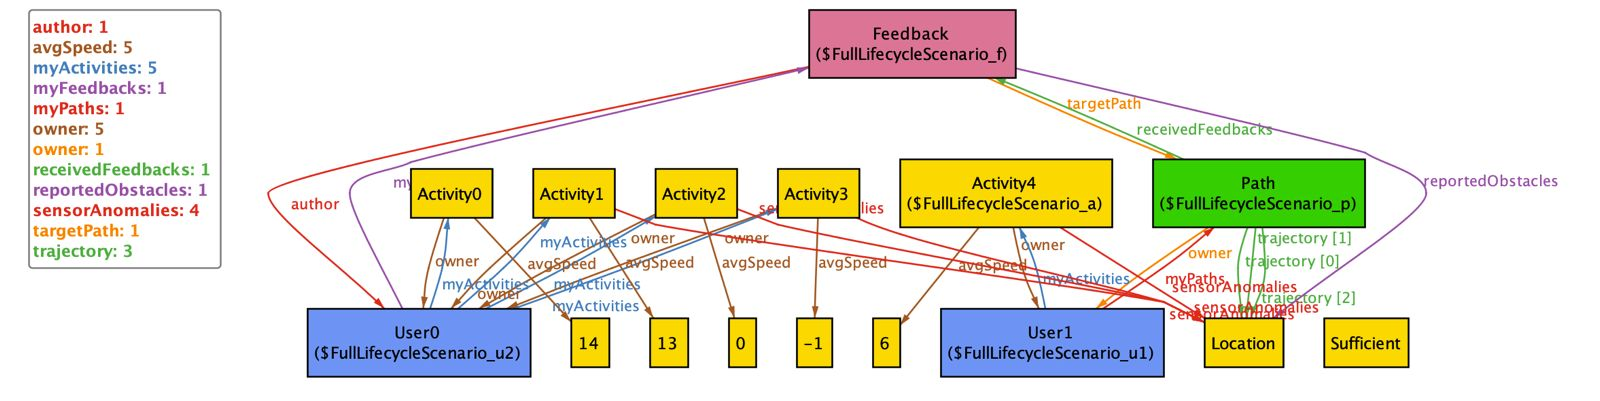
\includegraphics[width=0.8\textwidth]{Images/full_lifecycle_graph_1.jpeg} 
    \caption{Alloy instance: Full Lifecycle Scenario.}
    \label{fig:alloy_instance_1}
\end{figure}
\begin{figure}[H] % [H] forza l'immagine esattamente in questo punto
    \centering
    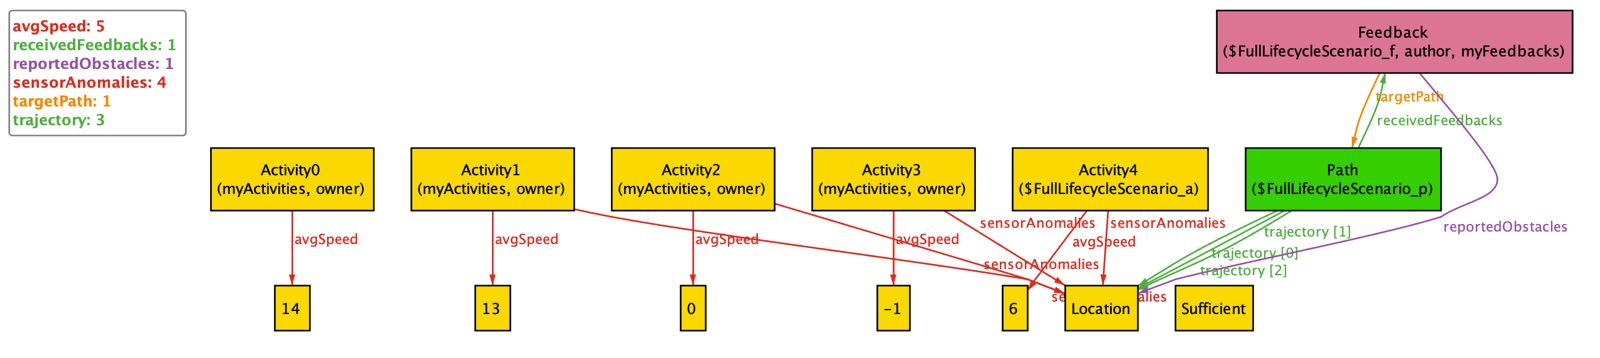
\includegraphics[width=0.8\textwidth]{Images/full_lifecycle_graph_2.jpeg} 
    \caption{Alloy instance: Full Lifecycle Scenario Projection User0.}
    \label{fig:alloy_instance_1}
\end{figure}
\begin{figure}[H] % [H] forza l'immagine esattamente in questo punto
    \centering
    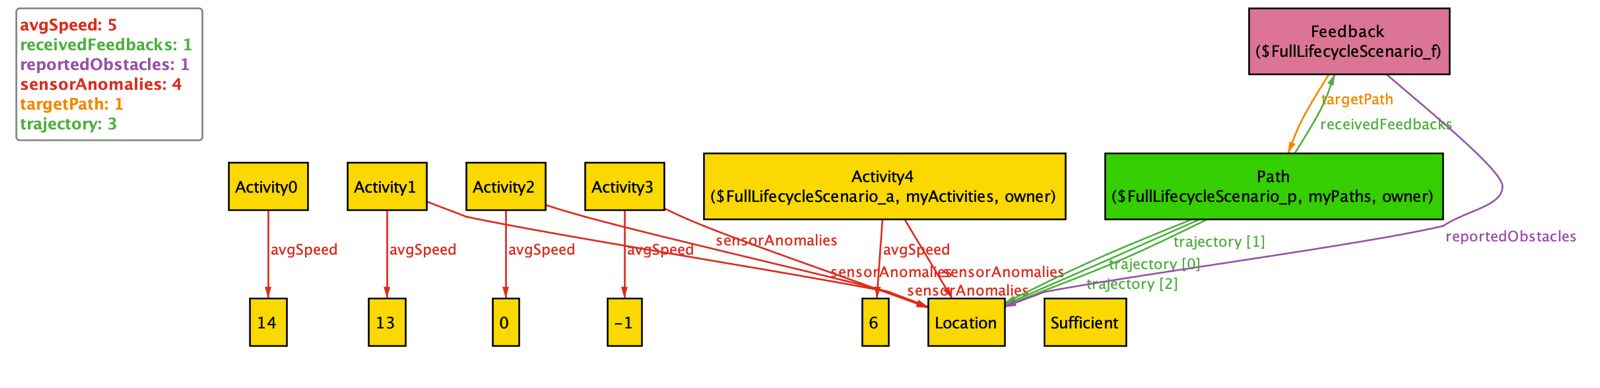
\includegraphics[width=0.8\textwidth]{Images/full_lifecycle_graph_3.jpeg} 
    \caption{Alloy instance: Full Lifecycle Scenario Projection User1.}
    \label{fig:alloy_instance_1}
\end{figure}

\section{Confliting Feedback Merge Scenario}

\begin{lstlisting}[language=Alloy, caption={Confliting Feedback Merge Scenario}, label={lst:alloy_model}]
    /* SCENARIO 2: CONFLICTING FEEDBACK MERGE
    Verifies that the system supports divergent opinions.
    Generates a public path with at least two feedbacks reporting 
    opposite conditions (e.g., Optimal vs Bad).
    */
    pred ConflictingFeedbackMerge {
        some p: Path | {
            p.status = Public
            #p.receivedFeedbacks >= 2
            some disj f1, f2: p.receivedFeedbacks | {
                f1.reportedCondition = Optimal
                f2.reportedCondition = Bad
            }
        }
    }
    run ConflictingFeedbackMerge for 4 but 5 Int
\end{lstlisting}

This scenario demonstrates the system's capability to handle and persist divergent opinions from the community regarding the same public path, a necessary condition for the merging logic.
The generated instance depicts a single Path with Public status linked to multiple distinct Feedback entities. Specifically, the model enforces the existence of conflicting reports, where one user rates the condition as Optimal while another rates it as Bad. 
This scenario formally validates the structural prerequisites for the Data Merging requirement. It proves that the domain model allows for the coexistence of contradictory data points without inconsistency. This accumulation of diverse feedback is the input required by the server-side aggregation algorithm to dynamically compute the path's overall score and \texttt{currentCondition}. 

\begin{figure}[H] % [H] forza l'immagine esattamente in questo punto
    \centering
    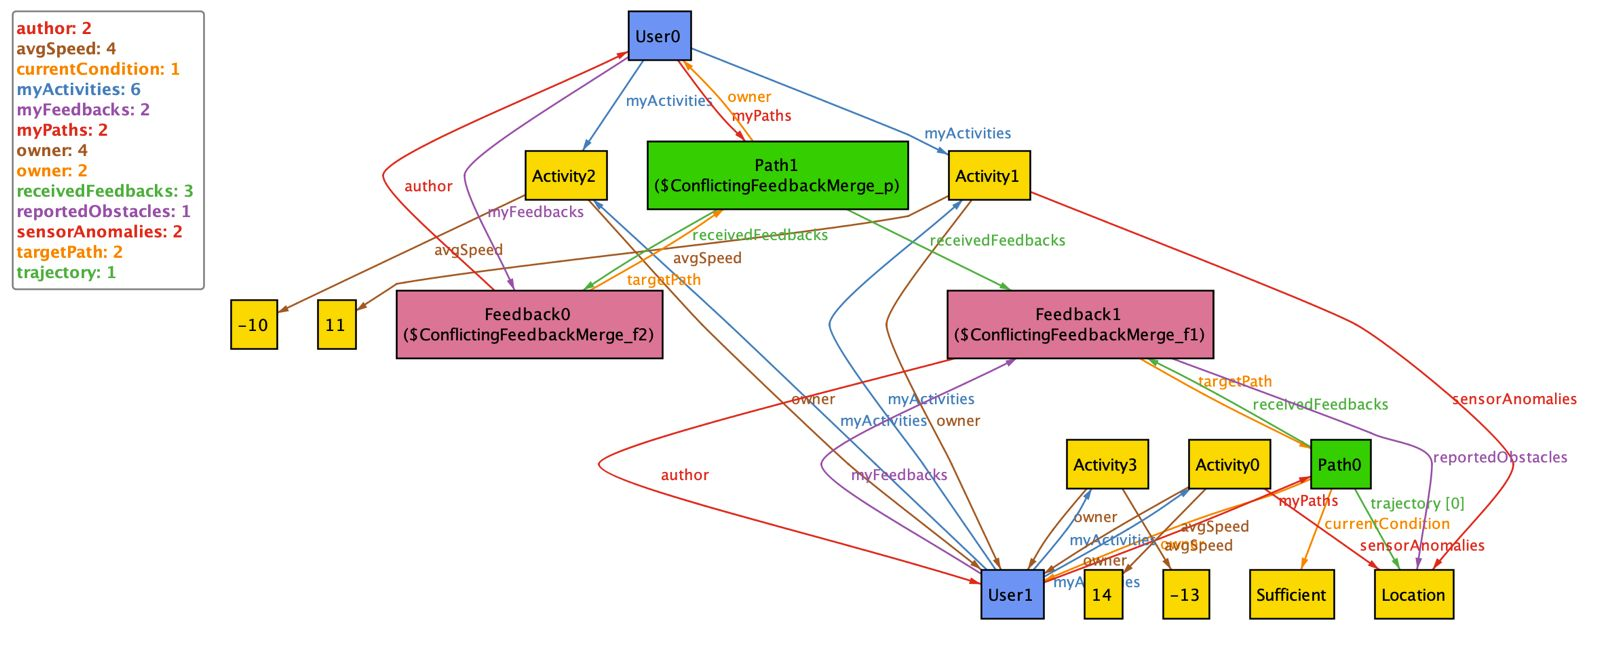
\includegraphics[width=0.8\textwidth]{Images/conflict_feedback_merge_graph.jpeg} 
    \caption{Alloy instance: Conflicting Feedback Merge Scenario.}
    \label{fig:alloy_instance_4}
\end{figure}

\section{Rejected Activity Filter Scenario}

\begin{lstlisting}[language=Alloy, caption={Rejected Activity Filter Scenario}, label={lst:alloy_model}]
/* SCENARIO 3: REJECTED ACTIVITY FILTER
   Demonstrates system robustness (Safety).
   Verifies the existence of an activity that is too slow (e.g., walking at speed 3)
   and ensures that NO path is generated from it.
*/
pred RejectedActivityScenario {
    some a: Activity | {
        a.avgSpeed = 3 
        
        no p: Path | p.owner = a.owner and p.trajectory = a.trace
    }
}
run RejectedActivityScenario for 3 but 5 Int
\end{lstlisting}

This scenario serves as a negative test to verify the robustness of the system's filtering logic, ensuring that invalid activities do not pollute the path database.
The predicate simulates an edge case where an Activity is recorded with an \texttt{avgSpeed} of 3 (representing a walking pace), which falls below the mandatory threshold defined in the domain facts (speed >4). The solver confirms that, in this state, no Path entity sharing the same trace and owner exists. 
This successfully verifies the Safety and Data Integrity constraints. It demonstrates that the logical rules correctly prevent the promotion of non-cycling activities (e.g., walking or running) into public paths, thereby guaranteeing that the platform remains focused exclusively on biking data. 

\begin{figure}[H] % [H] forza l'immagine esattamente in questo punto
    \centering
    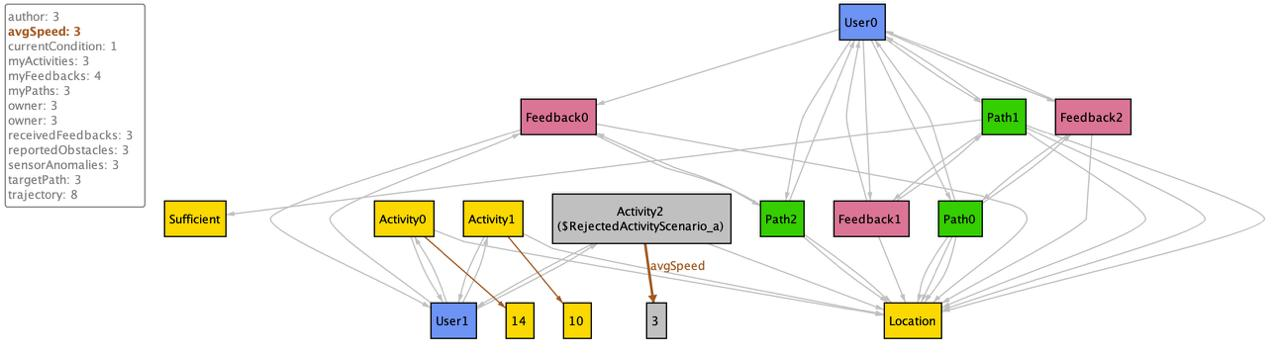
\includegraphics[width=0.8\textwidth]{Images/rejected_activity_graph.jpeg} 
    \caption{Alloy instance: Rejected Activity Scenario.}
    \label{fig:alloy_instance_5}
\end{figure}

%------------------------------------------------------------------------------------------------------------------------------------------------
\clearpage
\chapter{Effort Spent}
\label{sect:effort}
\begin{table}[h!]
\centering
\begin{tabular}{|l|c|c|c|}
\hline
\textbf{Data} & \textbf{Alessio Pesavento} & \textbf{Alberto Spezzapria} & \textbf{Luca Suzani} \\ 
\hline
27/10/2025 & 1h & 1h & 1h \\ 
\hline
07/11/2025 & 2h & 2h & 2h \\ 
\hline
08/11/2025 & - & 1h & - \\ 
\hline
09/11/2025 & 1h & - & - \\ 
\hline
\end{tabular}
\caption{Ore di lavoro per giorno e per membro del gruppo}
\label{tab:effort}
\end{table}


%------------------------------------------------------------------------------------------------------------------------------------------------



\end{document}
